% Данный файл распространяется под лицензией CC BY 4.0. Текст лицензии размещён на https://creativecommons.org/licenses/by/4.0/
% (c) Кафедра системного программирования, 2026

\documentclass[a4paper]{article}

\usepackage[a4paper, top=8mm, bottom=8mm, left=8mm, right=8mm]{geometry}

\usepackage{polyglossia}
\setdefaultlanguage[babelshorthands=true]{russian}
\setotherlanguage{english}

\usepackage{fontspec}
\setmainfont{FreeSerif}
\newfontfamily{\russianfonttt}[Scale=0.7]{DejaVuSansMono}

\usepackage[tiny, compact]{titlesec}

\usepackage{titling}
\setlength{\droptitle}{-1cm}
\pretitle{\centering\bfseries\Large}
\posttitle{\par}
\preauthor{\centering\normalsize}
\postauthor{\par\vspace{-1.8cm}}

\usepackage[hyphens]{url}
\usepackage{hyperref}
\usepackage[all]{hypcap}
\usepackage{bookmark}
\usepackage{csquotes}
\usepackage{booktabs}
\usepackage{graphicx}
\usepackage{float}
\usepackage{datetime2}
\usepackage{amsmath}


\title{Исследование масштабируемости и узких мест иерархии памяти в GPGPU архитектуре Vortex}

\author{Макухин Егор Александрович}

\date{}

\begin{document}

\raggedbottom
\emergencystretch=3em

\maketitle

\begin{flushright}
    Группа: \emph{25Б72-мм}

    Кафедра: \emph{Кафедра системного программирования}

    Научный руководитель: \emph{Григорьев Семён Вячеславович}
    
    Номер семестра практики: \emph{2}
\end{flushright} 

\section{Введение}

Работа выполняется в рамках исследования открытых GPGPU (General-Purpose Graphics Processing Unit~--- графических процессоров общего назначения) архитектур на базе набора команд RISC-V (Reduced Instruction Set Computer~V (пятое поколение))\footnote{The RISC-V Instruction Set Manual. URL: \url{https://riscv.org/technical/specifications/} (дата обращения: \DTMdate{2026-05-10}).}. Объектом исследования выступает проект Vortex\footnote{Vortex GPGPU Project. URL: \url{https://github.com/vortexgpgpu/vortex} (дата обращения: \DTMdate{2026-05-10}).}~--- открытая реализация GPGPU, предоставляющая полный RTL-код (Register Transfer Level~--- уровень регистровых передач), что позволяет проводить детальный архитектурный анализ в отличие от закрытых решений NVIDIA.

 \section{Постановка задачи}

\textbf{Целью работы является} проведение параметрического анализа конфигураций Vortex.

Для достижения цели были поставлены следующие задачи.
\begin{enumerate}
    \item Провести эксперименты сильного масштабирования (зависимость ускорения от количества вычислителей при фиксированном размере задачи).
    \item Разработать сценарий автоматизации для проведения параметрических экспериментов и извлечения метрик.
\end{enumerate}

Результаты работы необходимы для понимания архитектурных особенностей Vortex. Для исследователей архитектур и разработчиков это полезно тем, что позволяет избежать неэффективного использования ресурсов FPGA (Field-Programmable Gate Array~--- программируемая логическая интегральная схема) при конфигурации GPU для задач ограниченной вычислительной мощности и ограниченной пропускной способности памяти. В выполнении работы заинтересована кафедра для формирования рекомендаций по настройке экземпляров Vortex под различные классы задач.

\section{Описание предлагаемого решения}

В качестве среды моделирования используется программный симулятор \texttt{simx}\footnote{Software simulator simx of the Vortex project. URL: \url{https://github.com/vortexgpgpu/vortex/tree/master/sim/simx} (дата обращения: \DTMdate{2026-05-10}).}, входящий в состав проекта Vortex. Он выбран по причине высокой скорости работы по сравнению с полной RTL-симуляцией и отсутствия необходимости проведения синтеза для FPGA на ранних этапах оценки тенденций масштабирования. Важно отметить, что \texttt{simx} не является строго потактово точным, однако позволяет корректно оценивать относительные изменения производительности между конфигурациями.

Для достижения цели был предложен подход, основанный на автоматизированном тестировании модели Vortex с последующим извлечением метрик. Варьировались следующие параметры: количество вычислительных ядер, количество кластеров (групп вычислительных ядер, в кластере не более 4~--х ядер) и размер входных данных. Эксперименты проводились на задаче \texttt{sgemm} (умножение матриц одинарной точности)~--- задача с высокой вычислительной нагрузкой и высокой временной локальностью. Также при запуске экспериментов был использован флаг \texttt{perf} со значением 1, расширяющий количество выводимых метрик запуска.

Базовая конфигурация ядра была изменена. Изменённые параметры:
\begin{enumerate}
    \item \texttt{VX\_CFG\_NUM\_THREADS} = 32 (количество потоков исполнения на варп);
    \item \texttt{VX\_CFG\_NUM\_WARPS} = 32 (количество варпов на ядро, варп~--- минимальная единица планирования потоков в SIMD-архитектуре, Single Instruction Multiple Data~--- архитектуре с одним потоком команд и множеством потоков данных);
    \item \texttt{VX\_CFG\_L2\_ENABLE} = true (кэш L2);
    \item \texttt{VX\_CFG\_L3\_ENABLE} = true (кэш L3);
    \item \texttt{VX\_CFG\_L2\_SIZE} = 4194304 байт (размер кэша L2);
    \item \texttt{VX\_CFG\_L3\_SIZE} = 8388608 байт (размер кэша L3);
    \item \texttt{VX\_CFG\_DCACHE\_SIZE} = 131072 байт (размер кэша L1);
    \item \texttt{VX\_CFG\_DCACHE\_NUM\_WAYS} = 16 (количество каналов кэша L1);
    \item \texttt{VX\_CFG\_PLATFORM\_MEMORY\_NUM\_BANKS} = 16 (количество независимых банков (блоков) памяти).
\end{enumerate}

Для сборки конфигурации c 64~ядрами потребовалось расширить тип поля \texttt{num\_inputs} в структуре \texttt{Cache::Config} (файл sim/simx/mem/cache.h) с \texttt{uint8\_t} на \texttt{uint16\_t}, поскольку значение \texttt{VX\_CFG\_L3\_NUM\_REQS} при 64~ядрах достигает 256 и не помещается в \texttt{uint8\_t}. 

В качестве программного стека для разработки и запуска исследуемых параллельных приложений используется OpenCL (Open Computing Language~--- открытый язык вычислений на гетерогенных системах)\footnote{OpenCL~--- открытый стандарт параллельного программирования гетерогенных систем. URL: \url{https://www.khronos.org/opencl/} (дата обращения: \DTMdate{2026-05-10}).}. Написанные на OpenCL вычислительные ядра компилируются под архитектуру команд Vortex, а программный симулятор \texttt{simx} эмулирует их выполнение.


Реализация решения осуществлялась с использованием скриптов сборки Bash\footnote{Bash~--- командная оболочка UNIX-подобных систем. URL: \url{https://www.gnu.org/software/bash/} (дата обращения: \DTMdate{2026-05-10}).}, языка Python\footnote{Python~--- высокоуровневый язык программирования. URL: \url{https://www.python.org/} (дата обращения: \DTMdate{2026-05-10}).} для автоматизированного извлечения метрик из логов и визуализации данных (библиотеки pandas\footnote{pandas~--- библиотека Python для обработки и анализа данных. URL: \url{https://pandas.pydata.org/} (дата обращения: \DTMdate{2026-05-10}).} и matplotlib\footnote{matplotlib~--- библиотека Python для построения графиков. URL: \url{https://matplotlib.org/} (дата обращения: \DTMdate{2026-05-10}).}). Для обеспечения воспроизводимости результатов был разработан сценарий автоматизации, позволяющий запускать серию экспериментов одной командой.

\section{Эксперименты} 

Эксперименты проводились на ноутбуке Huawei MateBook 14 2024 под управлением операционной системы Ubuntu 24.04.4. Машина оснащена процессором Intel Core Ultra 5 125H (архитектура Meteor Lake, x86\_64) и 16~ГБ оперативной памяти LPDDR5X. Использовалась соответствующая коммиту 9540c33 версия проекта Vortex. Симулятор \texttt{simx} запускался в стандартном режиме без дополнительных флагов оптимизации. Использовалась версия Python 3.14.4,  а также библиотек pandas 3.0.2 и matplotlib 3.10.9.

В качестве основной метрики производительности используется количество тактов симулятора. Эта метрика выбрана потому, что она непосредственно отражает время выполнения задачи на архитектуре и позволяет однозначно сравнивать различные конфигурации между собой. Модель симулятора является детерминированной, поэтому результаты запусков воспроизводимы без статистического разброса.

На основе сформулированных задач были выделены следующие исследовательские вопросы (RQ~--- Research Questions).
\begin{enumerate}
    \item \textbf{RQ1:} влияет ли увеличение количества входных данных на масштабируемость задачи \texttt{sgemm}?
    \item \textbf{RQ2:} является ли масштабирование задачи \texttt{sgemm} линейным?
\end{enumerate}

\subsection{Модель исполнения задачи}
Вычислительная задача (сетка потоков) разбивается на независимые блоки потоков. Аппаратный планировщик распределяет готовые блоки целиком между доступными физическими ядрами GPU. Если количество сформированных блоков $N_{\text{blocks}}$ меньше числа физических ядер, то некоторые ядра не получают работы и остаются в состоянии простоя. Разбиение сетки и размер блока вычислялись автоматически функцией API Vortex \texttt{vx\_device\_max\_occupancy\_grid}. При конфигурации \texttt{VX\_CFG\_NUM\_WARPS = 32} и \texttt{VX\_CFG\_NUM\_THREADS = 32} функция устанавливала размер 2D~--блока в $32\times32$~потока ($1\,024$~потока на ядро). Соответственно, суммарное количество блоков в сетке рассчитывалось как $N_{\text{blocks}} = \left(\frac{N}{32}\right) \times \left(\frac{N}{32}\right) = \frac{N^2}{1024}$, что определяло число сформированных блоков для каждого размера задачи: $4$ блока при $N = 64$, $16$ блоков при $N = 128$, $64$ блока при $N = 256$ и $256$ блоков при $N = 512$.

\subsection{Обоснование параметров конфигурации и входных данных}

Выбор ключевых параметров экспериментальной установки и входных данных обусловлен архитектурными ограничениями Vortex GPGPU и принципами корректного методического анализа:
\begin{enumerate}
    \item \textbf{Ограничение размера кластера (до 4~ядер на кластер).} 
    Ограничение размера кластера 4~ядрами является стандартом для FPGA~--ориентированных GPGPU~--архитектур. Для масштабирования системы до 60~ядер используется 15 независимых 4~--ядерных кластеров.

    \item \textbf{Размеры входных матриц ($N = 64, 128, 256, 512$).} 
    Выбор размеров, кратных степеням двойки, обусловлен следующими факторами.
    \begin{enumerate}
        \item \textit{Кратность варпам.} Размер задачи $N$ во всех экспериментах кратна аппаратному размеру варпа архитектуры ($W = 32$). При стандартном разбиении сетки на блоки с размерностями, кратными степеням двойки, общее число потоков в блоке также оказывается кратным 32. Это гарантирует отсутствие частично заполненных варпов.
        \item \textit{Геометрический шаг нагрузки.} Каждая следующая степень двойки увеличивает суммарное число потоков $N^2$ ровно в 4 раза, что позволяет отслеживать переход системы от нехватки работы к полному насыщению.
    \end{enumerate}

    \item \textbf{Выбор исследуемых конфигураций ядер ($1, 2, 4, 8, 16, 32, 64$).} 
    Использование степеней двойки ($1, 2, 4, 8, 16, 32, 64$) необходимо для корректного анализа сильного масштабирования, так как общее число сформированных блоков потоков $N_{\text{blocks}}$ также кратно степеням двойки. Это гарантирует кратное и равномерное деление блоков между ядрами без простоя отдельных исполнителей.
\end{enumerate}

\subsection{Результаты масштабирования \texttt{sgemm}}

На рис.~\ref{fig:strong_sgemm_64}, \ref{fig:strong_sgemm_128}, \ref{fig:strong_sgemm_256} и \ref{fig:strong_sgemm_512} представлены графики масштабирования задачи \texttt{sgemm} в четырёх конфигурациях, задаваемых размерами матрицы: $64\times64$, $128\times128$, $256\times256$ и $512\times512$ элемента соответственно. По горизонтальной оси отложено количество ядер, по вертикальной~--- ускорение относительно конфигурации с одним ядром, для которой оно равно $1{,}0\times$. Ускорение является безразмерной величиной. Также на графике присутствует пунктирная линия, показывающая линейное масштабирование.

\begin{figure}[H]
    \centering
    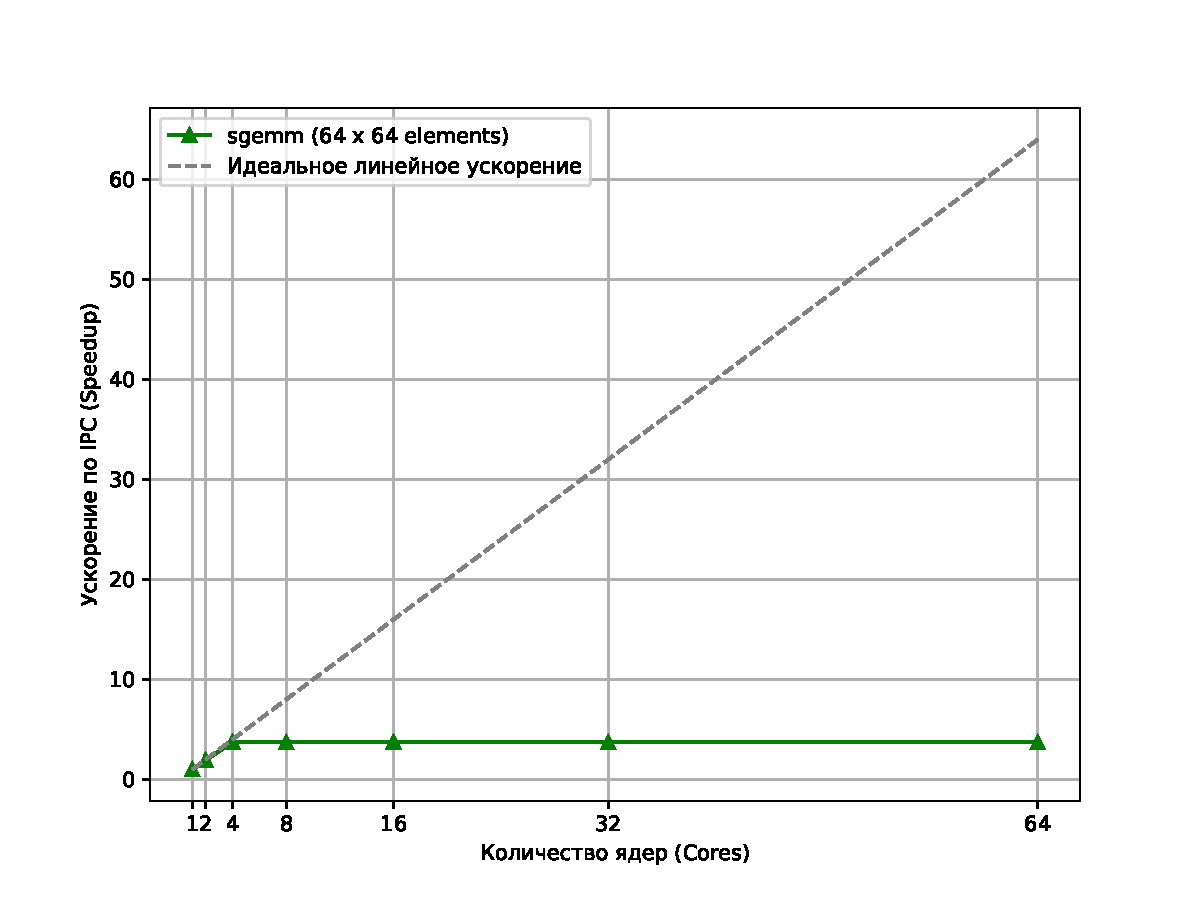
\includegraphics[width=0.85\textwidth]{images/strong_sgemm_64.pdf}
    \caption{Сильное масштабирование для задачи \texttt{sgemm} ($64\times64$)}
    \label{fig:strong_sgemm_64}
\end{figure}

\begin{figure}[H]
    \centering
    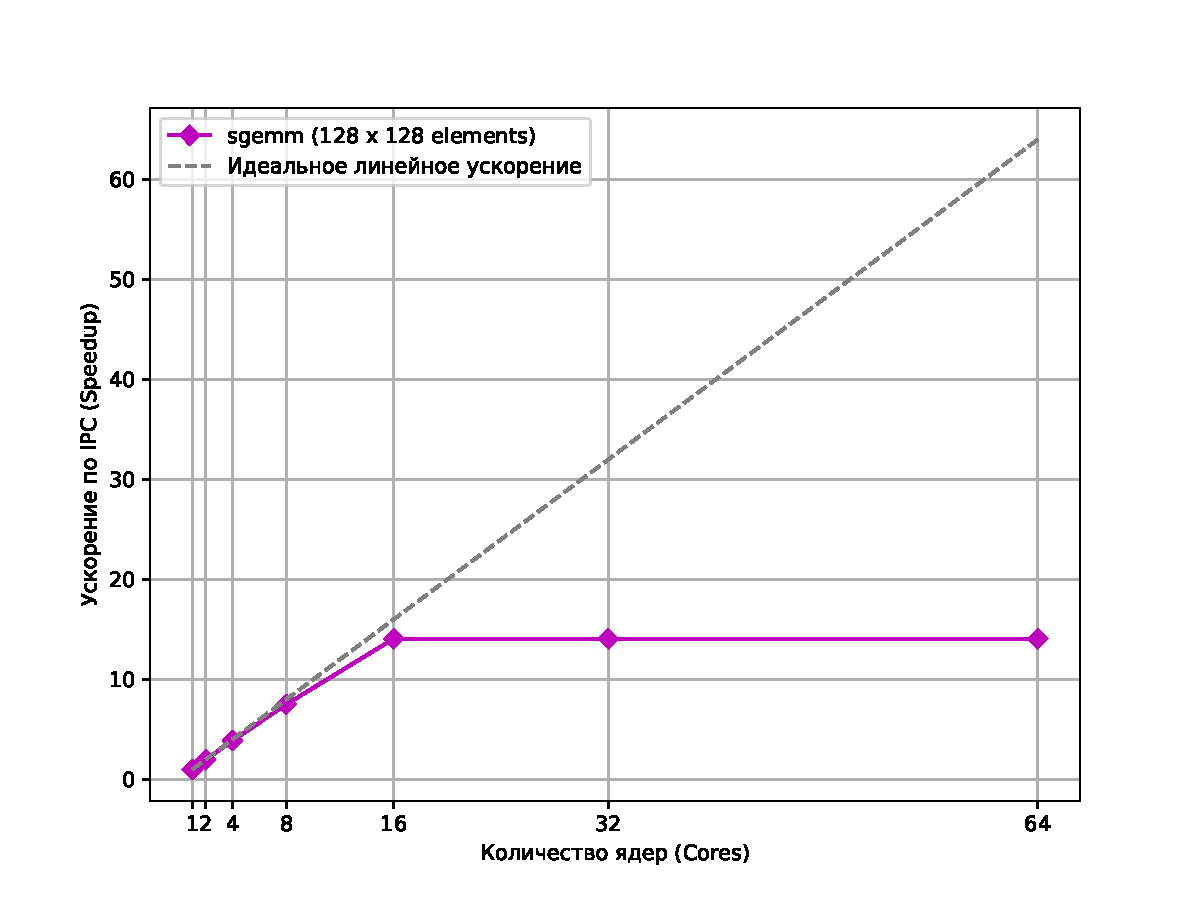
\includegraphics[width=0.85\textwidth]{images/strong_sgemm_128.pdf}
    \caption{Сильное масштабирование для задачи \texttt{sgemm} ($128\times128$)}
    \label{fig:strong_sgemm_128}
\end{figure}

\begin{figure}[H]
    \centering
    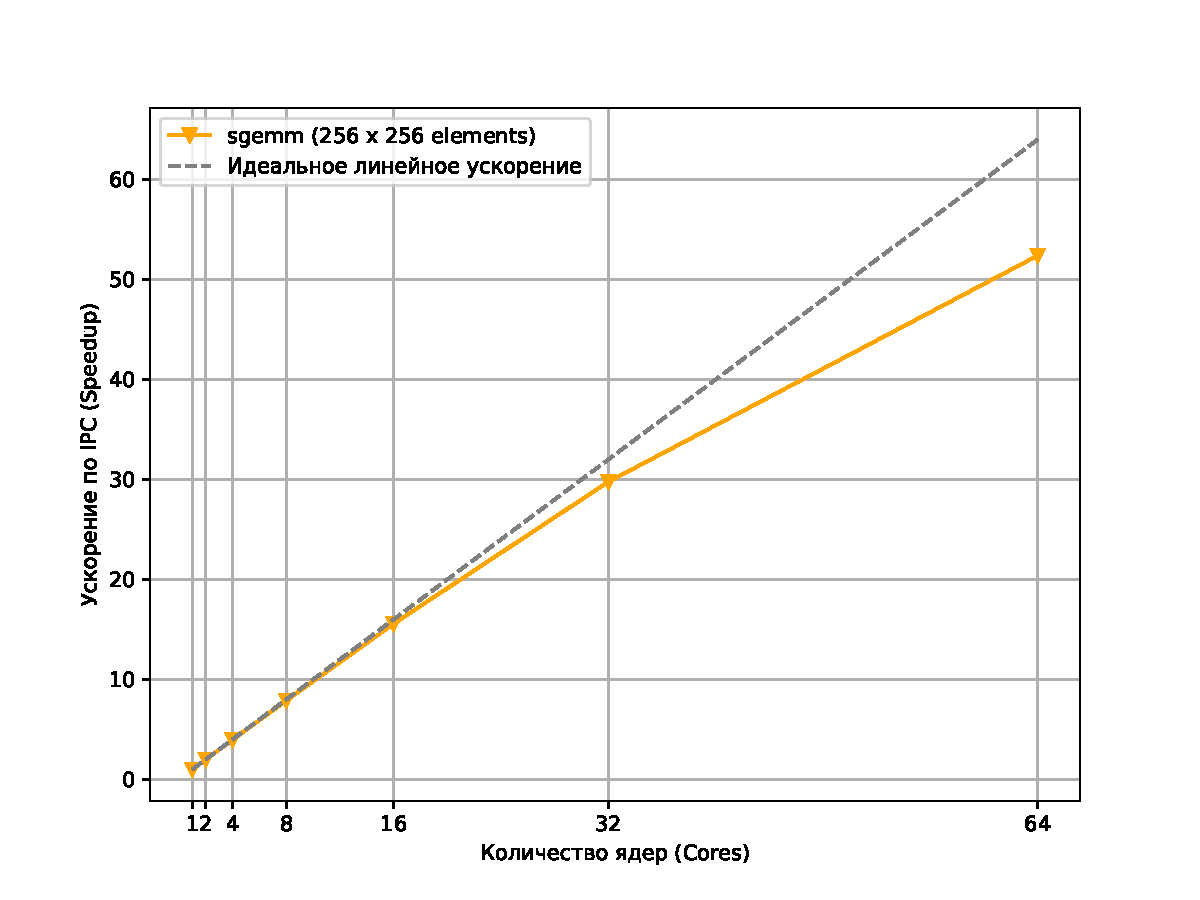
\includegraphics[width=0.85\textwidth]{images/strong_sgemm_256.pdf}
    \caption{Сильное масштабирование для задачи \texttt{sgemm} ($256\times256$)}
    \label{fig:strong_sgemm_256}
\end{figure}

\begin{figure}[H]
    \centering
    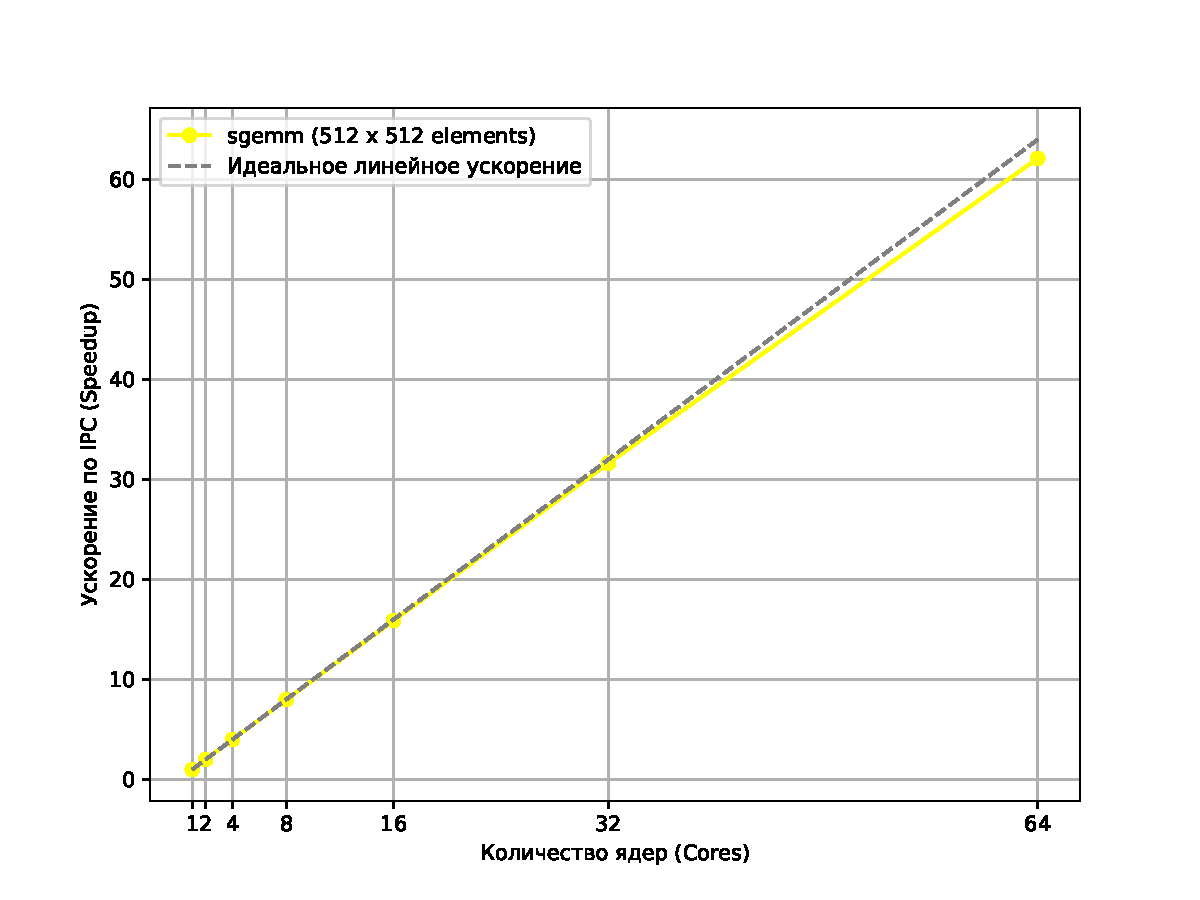
\includegraphics[width=0.85\textwidth]{images/strong_sgemm_512.pdf}
    \caption{Сильное масштабирование для задачи \texttt{sgemm} ($512\times512$)}
    \label{fig:strong_sgemm_512}
\end{figure}

\textbf{Аппаратно-программная база задачи \texttt{sgemm}.}
Формирование сетки вычислений определяется взаимодействием хост-кода (\texttt{main.cpp}) и ядра (\texttt{kernel.cpp}). В \texttt{main.cpp} вычисляются размеры блока и сетки для заданной глобальной размерности задачи с помощью функции \texttt{vx\_device\_max\_occupancy\_grid}.

\begin{verbatim}
const uint32_t global_dim[2] = {size, size};
CHECK(vx_device_max_occupancy_grid(dev, 2, global_dim, grid, block));
\end{verbatim}

В ядре каждый поток рассчитывает ровно один элемент итоговой матрицы $C[row][col]$.

\begin{verbatim}
int col = blockIdx.x * blockDim.x + threadIdx.x;
int row = blockIdx.y * blockDim.y + threadIdx.y;

#pragma unroll 8
for (uint32_t e = 0; e < size; ++e) {
sum += A[row * size + e] * B[e * size + col];
}
C[row * size + col] = sum;
\end{verbatim}

Директива \texttt{\#pragma unroll 8} разворачивает внутренний цикл на 8~итераций, что увеличивает число одновременных запросов к памяти от одного варпа.

Таким образом, общее число параллельных потоков в системе строго равно $N^2$, где $N$~--- размер одной оси квадратной матрицы.

\textbf{Анализ результатов сильного масштабирования.}
\begin{enumerate}
    \item \textbf{$N = 64$.} 
    При $N = 64$ количество потоков $N^2 = 4\,096$, что при блоке $32 \times 32$ дает всего $N_{\text{blocks}} = 4$~блока (сетка $2 \times 2$). Сформированных блоков хватает для загрузки лишь 4~ядер (по 1~блоку на ядро). При увеличении числа ядер до 8, 16 и 32 количество физических ядер превышает число блоков. Ядра, не получившие блоков для выполнения, остаются в состоянии простоя, что останавливает рост ускорения на уровне 4~ядер. 

    \item \textbf{$N = 128$.} 
    Объём $N^2 = 16\,384$~потока формирует $N_{\text{blocks}} = 16$~блоков ($4 \times 4$), позволяя загрузить ровно 16~ядер. При 32~ядрах половина ядер простаивает из-за дефицита блоков (16~блоков на 32~ядра).

    \item \textbf{$N = 256$.} 
    При $N^2 = 65\,536$~потоках задача разбивается на $N_{\text{blocks}} = 64$ блока ($8 \times 8$). Объёма работы достаточно для линейного масштабирования, однако график близок к нему только до 32~ядер (ровно по 2~блока или $2\,048$~потока на ядро, ускорение $30\times$). При переходе к 64~ядрам график ложится ниже линии линейного масштабирования не из-за дефицита блоков как в предыдущих задачах (их ровно 64, по одному на ядро), а из-за роста задержки памяти: значение метрики \texttt{load\_lat}, показывающей среднюю задержку в тактах между выдачей запроса на чтение из памяти и получением данных, увеличивается с $25{,}77$~такта на одном ядре до $49{,}82$~такта при 64~ядрах. Это означает, что памяти стало сложнее успевать отдавать данные из-за большого количества одновременно обращающихся к ней ядер.
    
    \item \textbf{$N = 512$.} 
    Размер $N^2 = 262\,144$~потоков формирует $N_{\text{blocks}} = 256$~блоков ($16 \times 16$), обеспечивая высокую плотность работы. На каждое из 64~ядер приходится $4$~блока ($4\,096$~потоков на ядро). Это позволяет сохранять линейный уровень масштабирования и достигать ускорения $\approx 63{,}0\times$ на 64~ядрах.
\end{enumerate}

\textbf{Вывод из экспериментов задачи \texttt{sgemm}.}
Масштабируемость архитектуры Vortex зависит от количества сформированных блоков ($N_{\text{blocks}}$), определяющих предел загрузки ядер.
Точки насыщения вычислительных ресурсов:
\begin{enumerate}
    \item $N = 64$ ($4\,096$~потоков)~--- максимум 4~ядра (всего $N_{\text{blocks}} = 4$~блока, остальные ядра простаивают);
    \item $N = 128$ ($16\,384$~потока)~--- максимум 16~ядер (дефицит блоков: $N_{\text{blocks}} = 16$, из-за чего 16 из 32~ядер простаивают);
    \item $N = 256$ ($65\,536$~потоков)~--- эффективно до 64~ядер (ровно по 1~блоку на ядро), однако при 64~ядрах наблюдается небольшое отклонение от линейного масштабирования из-за конкуренции между ядрами за обращения к памяти.
    \item $N = 512$ ($262\,144$~потока)~--- сохраняет близкую к линейной масштабируемость на всех 64~ядрах ($N_{\text{blocks}} = 256$~блоков, ускорение $\approx 63{,}0\times$).
\end{enumerate}

\section{Заключение}

В ходе выполнения работы получены следующие результаты.
\begin{enumerate}
    \item Разработан сценарий автоматизации\footnote{Репозиторий на Github с исходным кодом сценария автоматизации. URL: \url{https://github.com/Makuhin-Egor/Vortex-experiments-styding-practice} (дата обращения: \DTMdate{2026-05-10}).} (Bash + Python) для извлечения метрик из логов и визуализации результатов, обеспечивающий воспроизводимость исследования.
    \item Проведены эксперименты сильного масштабирования, в ходе которых получен ответ на исследовательские вопросы.
    \begin{enumerate}
        \item \textbf{RQ1:} увеличение количества входных данных влияет на масштабируемость задачи \texttt{sgemm}. 
        \item \textbf{RQ2:} масштабирование задачи \texttt{sgemm} является линейным в том случае, если количества блоков, на которые она разбивается, достаточно для загрузки всех ядер и при этом их количество кратно количеству ядер.
    \end{enumerate}
\end{enumerate}

\end{document}